\documentclass[10pt,journal,cspaper,compsoc]{IEEEtran}
%
% If IEEEtran.cls has not been installed into the LaTeX system files,
% manually specify the path to it like:
% \documentclass[12pt,journal,compsoc]{../sty/IEEEtran}

\usepackage{fixltx2e}
% \usepackage{stfloats}
\usepackage{amsmath}
\usepackage{graphicx}
\usepackage{amsfonts}
\usepackage{amsthm}
\usepackage{cite}
\usepackage{algorithm}
\usepackage{algorithmic}
\usepackage{url}
\input{/Users/jovo/Research/latex/latex_commands.tex}
\hyphenation{op-tical net-works semi-conduc-tor}


\begin{document}

\title{Graph Classification using Signal Subgraphs: Applications in Statistical Connectomics}

\author{Joshua T.~Vogelstein,
		William~R.~Gray,
        R.~Jacob~Vogelstein,
        and~Carey~E.~Priebe% <-this % stops a space
\IEEEcompsocitemizethanks{\IEEEcompsocthanksitem J.T. Vogelstein and C.E. Priebe are with the Department
of Applied Mathematics and Statistics, Johns Hopkins University, Baltimore, MD 21218.\protect\\
% note need leading \protect in front of \\ to get a newline within \thanks as
% \\ is fragile and will error, could use \hfil\break instead.
E-mail: joshuav@jhu.edu
\IEEEcompsocthanksitem W.R. Gray and R.J. Vogelstein are with the Johns Hopkins University Applied Physics Laboratory, Laurel, MD, 20723.}% <-this % stops a space
\thanks{}}
 
% The paper headers
\markboth{IN PREP}%
{Graph Classification}

\IEEEcompsoctitleabstractindextext{%
\begin{abstract}
%\boldmath
In this manuscript, we consider the following ``graph classification'' question: given a collection of graphs and associated classes, how can we predict the class of a newly observed graph?  To address this question we propose a statistical model for graph/class pairs.  Given this model, we devise a set of estimators to identify the class-conditional signal, referred to here as the ``signal subgraph.'' The classifiers differ by their assumption about the ``coherency'' of the signal subgraph, that is, the minimum number of vertices to which all signal subgraph edges are incident. The best estimator is shown to be not just a function of the coherency of the model, but also the number of training samples.  These estimators are employed on an interesting neuroscience question: can we classify connectomes according to sex?  The answer is yes, and significantly better than a na\"ive strategy.  Synthetic data analysis demonstrates that even when model is correct, given the relatively small number of training samples, the estimated signal subgraph should be taken with a grain of salt.  We conclude by discussing several possible extensions.
\end{abstract}

% Note that keywords are not normally used for peer review papers.
\begin{keywords}
statistical inference, graph theory, network theory, structural pattern recognition, connectome, classification.
\end{keywords}}


% make the title area
\maketitle
\IEEEdisplaynotcompsoctitleabstractindextext
\IEEEpeerreviewmaketitle



\section{Introduction}

\IEEEPARstart{G}{raphs} are becoming increasingly popular vehicles for data representation, spanning fields from optical character recognition and chemistry \cite{Bunke2011} to neuroscience \cite{Hagmann2010}.  While statistical inference techniques for vector-valued data are widespread, statistical tools for the analysis of graph-valued data are relatively rare \cite{Bunke2011}. In this work we consider the task of \emph{graph classification}: given a collection of graphs and their corresponding classes, can we accurately estimate the class of a new graph lacking a class label?  We propose and analyze a joint graph/class model---sufficiently simple to characterize its asymptotic properties, and sufficiently rich to afford useful empirical applications.  This model admits a class-conditional signal encoded in a subset of edges, the \emph{signal subgraph}. Finding the signal subgraph amounts to providing an understanding of the differences between the two graph classes.  Moreover, we are interested in learning to what extent this signal is ``coherent'', that is, to what extent all of the edges are incident to a relatively small set of vertices.  This approach is qualitatively different from most previous approaches which utilize only (i) vertex labels or (ii) graph structure.  More specifically, simply representing the adjacency matrix with a vector and apply standard machine learning techniques ignores graph structure.  Alternately, computing a set of graph invariants (such as clustering coefficient), and then classify using only these invariants ignores vertex labels.  Neither of these approaches use both vertex labels and graph structure.  We demonstrate via theory, simulation, analysis of a neurobiological data set (magnetic resonance based connectomes), and synthetic data analysis, that utilizing graph structure can significantly enhance classification accuracy.  However, the best approach for any particular data set is not just a function of the model, but also the amount of data.  Moreover, even when the model is true, given a relatively small sample size, the estimated signal subgraph will often overlap with the truth, but not fully capture it.  Nonetheless, the classifiers described below still significantly outperform the benchmarks.

\section{Methods} % (fold)
\label{sec:methods}

% section methods (end)

\subsection{Setting}

Let $\GG: \Omega \mapsto \mc{G}$ be a graph-valued random variable with samples $G_i$.  Each graph is defined by a set of $V$ vertices, $\mc{V}=\{v_i\}_{i \in [V]}$, where $[V]=\{1,\ldots, V\}$, and a set of possible edges between pairs of vertices $\mc{E}$, where $|\mc{E}| \leq V^2$. An adjacency matrix, $A$, is a binary $V \times V$ matrix identifying which vertices share an edge. Let $Y:\Omega \mapsto \mc{Y}$ be a discrete-valued random variable with samples $y_i$.  Assume the existence of a collection of $n$ exchangeable samples of graphs and their corresponding classes from some true but unknown joint distribution: $\{(\GG_i,Y_i)\}_{i \in [n]} \overset{exch.}{\sim} F_{\GG,Y}$. Our aim (or exploitation task) is to build a graph classifier that can take a new graph, $g$, and correctly estimate its class, $y$, assuming that they are jointly sampled from the same distribution, $F_{\GG,Y}$.  Moreover, we are interested solely in graph classifiers that are \emph{interpretable} with respect to the vertices and edges of the graph. In other words, manifold learning, feature extraction, and related approaches are inadmissible.  

\subsection{Model} % (fold)
\label{sub:model}

A model defines the set of distributions under consideration.  In the graph classification domain, we consider the model, $\mc{F}_{\GG,Y}$, which includes all joint distributions over graphs and classes under consideration: $\mc{F}_{\GG,Y}=\{F_{\GG, Y}(\cdot; \bth) : \bth \in \bTh\}$, where $\bth \in \bTh$ indexes each distribution.  Two ``standard'' approaches for tackling a classification problem are (i) the \emph{generative} approach and (ii) the \emph{discriminative} approach.  In a generative strategy, one decomposes the joint distribution into a product of a likelihood term and a prior term:  $F_{\GG,Y}=F_{\GG | Y}F_Y$.  In a discriminative strategy, one decomposes the joint distribution into a posterior term and a marginal term: $F_{\GG,Y}=F_{Y | \GG}F_{\GG}$.  We proceed using a hybrid generative-discriminative approach whereby we describe a generative model and place constraints on the discriminant boundary.

First,  assume that each graph has the same set of labeled vertices, so that all the variability in the graphs is in the adjacency matrix, which implies that $F_{\GG,Y}=F_{A,Y}$. Second, assume edges are independent, that is: $F_{A,Y}=\prod_{u,v \in \mc{E}} F_{A_{uv},Y}$.  Now, consider the generative decomposition, and let $F_{uv|y}=F(A_{uv} | Y=y)$ and $\pi_y=F_{Y=y}$.  Third, assume the existence of a class-conditional difference, that is $F_{uv|0} \neq F_{uv|1}$ for some $(u,v) \in \mc{E}$, and denote the edges satisfying this condition  the \emph{signal subgraph}, $\mc{S}=\{(u,v) \in \mc{E}: F_{uv|0} \neq F_{uv|1}\}$.  Fourth, for concreteness, assume that the graphs are \emph{simple} graphs, that is, undirected, with binary edges, and lacking (self-) loops.  Thus, the likelihood of an edge between vertex $u$ and $v$ is given by a Bernoulli random variable with a scalar probability parameter:  $F_{uv|y}=\text{Bern}(A_{uv}; p_{uv|y})$. Together, these four assumptions imply the following model: 
\begin{equation}
\mc{F}_{\GG,Y}=\{F_{A, Y}(a,y; \bth) \quad \forall a\in\mc{A},y\in\mc{Y}: \bth \in \bTh\},
\end{equation} 
such that
\begin{multline}
F_{A,Y}(a,y; \theta) =  \prod_{uv \in \mc{S}} \text{Bern}(a_{uv}; p_{uv|y})  \pi_y 
\\ \times \prod_{uv \in \mc{E} \backslash \mc{S}} \text{Bern}(a_{uv}; p_{uv}),
\end{multline}
where $\bth=\{\mb{p},\mb{\pi},\mc{S}\}$. The likelihood parameter is constrained such that each element must be between zero and one: $\mb{p}\in (0,1)^{V\times V \times |\mc{Y}|}$.  The prior parameter, $\mb{\pi}=(\pi_1, \ldots, \pi_{|\mc{Y}|})$, must have elements greater than or equal to zero and sum to one: $\pi_y \geq 0, \sum_y \pi_y=1$.  The signal subgraph parameter is a non-empty subset of the set of possible edges, $\mc{S} \subseteq \mc{E}$ and $\mc{S} \neq \emptyset$.

We consider up to two additional constraints on $\mc{S}$.  First, the size of the signal subgraph may be constrained such that $|\mc{S}| \leq s$. Second, the minimum number of vertices onto which each edge is incident is constrained such that $\mc{S}=\{(u,v): u \in \mc{U} \cup v \in \mc{U}\}$, where $\mc{U}$ is a set of \emph{signal vertices} with $|\mc{U}|\leq m$. Edges in the signal subgraph are called \emph{signal edges}. 

Note that given a specification of the class-conditional likelihood of each edge and class-prior, one completely defines a possible joint distribution over graphs and classes; the signal subgraph is implicit in that parameterization. However, the likelihood parameters for all edges not in the signal subgraph, $p_{uv|y}=p_{uv} \, \forall \, y \in \mc{Y}, (u,v) \notin \mc{S}$,  are \emph{nuisance} parameters; that is, they contain no class-conditional signal.  Note that when computing a relative posterior class estimate, these nuisance parameters cancel in the ratio.



% subsection model (end)

\subsection{Classifier} % (fold)
\label{sub:classifier}



Formally, we say that a graph classifier, $h \in \mc{H}$, is any function satisfying $h: \mc{G} \mapsto \mc{Y}$.  We desire to obtain the ``best'' possible classifier, $h_*$. To define best, we first define a loss function, $\ell_h: \mc{G} \times \mc{Y} \mapsto \Real_+$, specifically the $0-1$ loss function:
\begin{align}
\ell_h(G,Y) \defeq \II \{h(G) \neq Y\}, %=\\ \int
% _{g \in \mc{G}, y\in \mc{Y}} 
%F[h(g) \neq y] F[g,y] dgdy.
\end{align}
where $\II\{\cdot\}$ is the indicator function, equaling one whenever its argument is true, and zero otherwise.  Further, let risk, $R: \mc{F} \times \mc{H} \mapsto \Real_+$ be the expected loss under the true distribution:
\begin{align}
R(F,h) \defeq \EE_F[\ell_h(G,Y)].
\end{align}
We define the best (optimal) classifier for a given distribution $F$ as the one that minimizes risk.
%(under model $\mc{F}$ and loss-function $\ell$) as the classifier with minimal expected loss: $h_*=\argmin_{h \in \mc{H}} \EE_F [\ell (F,Y)] \forall F \in \mc{F}$.  Such a classifier is called \emph{Bayes optimal}, and the error associated with such a classifier is called \emph{Bayes error} or \emph{Bayes risk}.  
It can be shown that the classifier that maximizes the class-conditional posterior, $F_{Y | \GG}$ is optimal \cite{Bickel2000}:
\begin{align} \label{eq:map}
h_*(G) &= \argmin_{h \in \mc{H}} \EE_F[\ell_h (G,Y)] %= \argmax_{Y \in \mc{Y}} F_{Y|G} 
\nonumber \\ &= \argmax_{y \in \mc{Y}} F_{G|Y=y} F_{Y=y}.
\end{align}
Given the proposed model, Eq. \eqref{eq:map} can be further factorized using the above four assumptions:
\begin{align}
h_*(G)
% \argmax_{Y \in \mc{Y}} F_{G|Y} F_Y 
% &= \argmax_{y \in \mc{Y}} F[a|y] F[y] 
% \nonumber \\ &= \argmax_{y \in \mc{Y}} \prod_{u,v \in \mc{E}} F_{uv | y} \pi_y 
% \nonumber \\ &= \argmax_{y \in \mc{Y}} \prod_{u,v \in \mc{S}} F_{uv | y} \pi_y 
% \nonumber \\ 
&= \argmax_{y \in \mc{Y}} \prod_{u,v \in \mc{S}} \text{Bern}(A_{uv}; p_{uv|y}) \pi_y.
\end{align}
Unfortunately Bayes optimal classifiers are typically unavailable. In such settings, it is therefore desirable to induce a classifier estimate from a set of \emph{training data}. Formally, let $\mc{T}_n= \{(\GG_i,Y_i)\}_{i \in [n]}$ denote the training corpus, where each graph-class pair is sampled exchangeably from the true but unknown distribution: $(\GG_i,Y_i) \overset{exch.}{\sim} F_{\GG, Y}$.  Given such a training corpus, and an unclassified graph, $g$, an induced classifier predicts the true (but unknown) class of $g$ by utilizing the training corpus: $\mt{h}: \mc{G} \times (\mc{G} \times \mc{Y})^n \mapsto \mc{Y}$.  When a model $\mc{F}_{\GG,Y}$ is specified, a beloved approach is to use a  \emph{Bayes plugin classifier}. Due to the above simplifying assumptions, the Bayes plugin classifier for this model is defined as follows.  First, estimate the  model parameters: $\bth=\{\mc{S}, \mb{p}, \mb{\pi}\}$. Second, plug those estimates into the above equation.  The result is a Bayes plugin graph classifier:
\begin{align}
\mt{h}(g; \mc{T}_n) \defeq  \argmax_{y \in \mc{Y}} \prod_{u,v \in \mhc{S}}
\mh{p}_{uv|y}^{a_{uv}}(1-\mh{p}_{uv|y})^{(1-a_{uv})} \mh{\pi}_y,
\end{align}
where the Bernoulli probability is explicit. To implement such a classifier estimate, we specify estimators for $\mc{S}$, $\mb{\pi}$ and $\mb{p}$.

% subsection classifier (end)

\subsection{Estimators} % (fold)
\label{sub:estimators}


In this section we describe estimators to estimate the estimands (parameters) of our model.  An \emph{estimator} is a function that maps from the multiple-sample space to the parameter space: $\bhth_n: \Xi^n \mapsto \bTh$; the output of this function is called the \emph{estimate}.  In the graph classification domain, for example, $\Xi=(\mc{G},\mc{Y})$.  In a slight abuse of notation, we will also refer to the sequence of estimators, $\bhth_1,\bhth_2, \ldots$, as an estimator.  We desire (a sequence of) estimators that satisfy the following desiderata:

\begin{itemize}
	\item \textbf{Consistent}: an estimator is consistent if its sequence converges in the limit to the true value: $\lim_{n \conv \infty} \bhth_n = \bth$.  %When the parameter is multidimensional, an estimator can be consistent as the number of samples $n$ goes to infinity (i) but the dimensionality is fixed at $d$, or (ii) the dimensionality also goes to infinity.  The estimate resulting from using a consistent estimator is called \emph{asymptotically unbiased}.
	\item \textbf{Efficient}: an estimator is efficient if its sequence converges to the %minimum variance: $\lim_{n\conv\infty} \text{Var}(\bhth_n) = \mc{I}_{\bth}^{-1}$.  %If one allows for infinite dimensional parameters, than it might be desirable to compute efficiency as both $n$ and $d$ approach infinity.  
	% An efficient estimator yields an estimate with 
	\emph{minimum variance}.
	\item \textbf{Robust}: an estimator is robust if the resulting estimate is relatively insensitive to small model misspecifications.  Because the space of models is massive (uncountably infinite), it is intractable to consider all misspecifications, so we only consider a few of them, as described below.
	\item \textbf{Quadratic complexity}: computational time complexity should be quadratic in the number of vertices or less.
	\item \textbf{Interpretable}: we desire that the parameters are interpretable with respect to a subset of vertices and/or edges.
\end{itemize}
In addition to the above categorical desiderata, we also desire ``nice'' finite sample and empirical performance.


\subsubsection{Signal Subgraph Estimators} % (fold)
\label{ssub:subsubsection_name1}


Na\"{i}vely, one might consider a search over all possible signal subgraphs, by plugging each one in to the classifier, and selecting the best performing option.  This strategy is intractable because the number of signal subgraphs scales super-exponentially with the number of vertices (see Figure \ref{fig:numgraphs}, left panel). Specifically, the number of edges in a simple graph with $V$ vertices is $d_V=\binom{V}{2}$, so the number of unique subgraphs is $2^{\binom{V}{2}}$.  Searching over all of them is therefore ridiculously computationally taxing, failing the quadratic complexity criterium (it would even fail an exponential complexity criterium). %Second, the estimate will be determined partially by the chosen classifier.  This makes interpreting the results a bit tricky, because if one uses two different classifiers and as one cannot ascertain whether the signal subgraph chosen is the one that works best for the chosen classifier, or is the true signal subgraph (assuming that they could be different).  
We therefore consider several alternatives.


% subsubsection subsubsection_name (end)



\begin{figure*}[tb!]
	\centering
		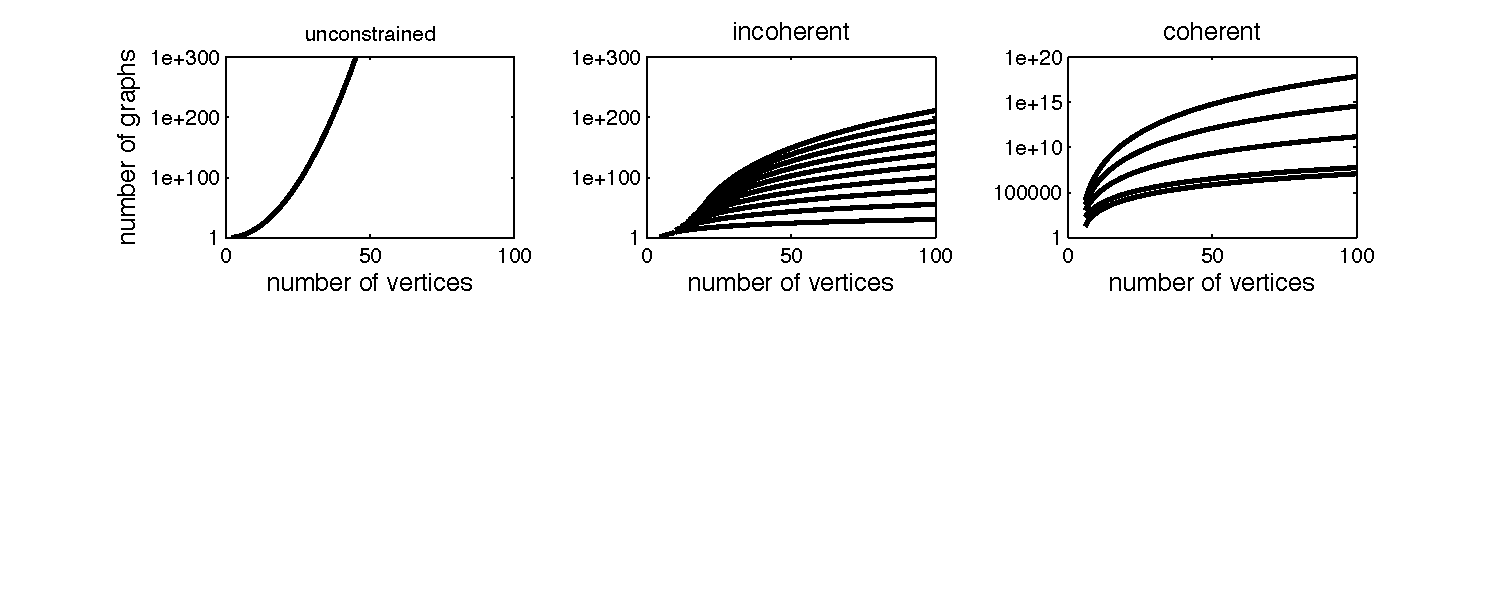
\includegraphics[width=1.0\linewidth]{../figs/num_of_graphs.pdf}
	\caption{Exhaustive searches for the signal subgraph, even given severe constraints, are computationally intractable for small graphs (e.g., with $\mc{O}(10)$ vertices).  Top panels show the number of unique simple subgraphs as a function of the number of vertices, $V$.  Note the ordinates are all log scale.   On the left is the unconstrained scenario, that is, all possible subgraphs for a given number of vertices.  In the middle panel, each line shows the number of subgraphs with fixed number of signal edges, $s$, ranging from 10 to 100, incrementing by 10 with each line.  The right panel shows the number of subgraphs for various fixed $s$ and only a single signal vertex, that is, all edges are incident to one vertex.  Bottom panels show a particular example subgraph via its adjacency matrix; white elements indicate an edge.}
	\label{fig:numgraphs}
\end{figure*}

\begin{figure*}[tb!]
	\centering
		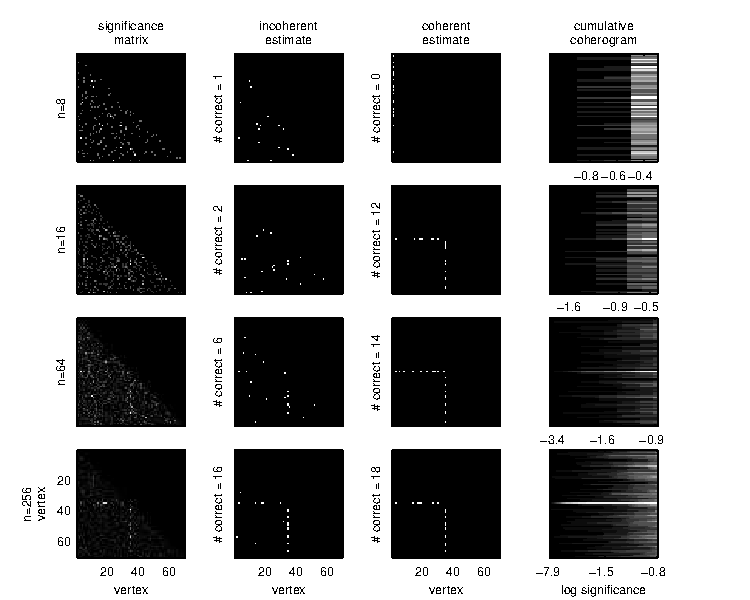
\includegraphics[width=1.0\linewidth]{../figs/homo_V70_s20_p10_q30_SigIncCohErogram.pdf}
	\caption{An example of the coherent signal subgraph estimate's improved accuracy over the incoherent signal subgraph estimate, for a particular homogeneous two-class model specified by: $\mc{M}_{70}(1,20;0.5,0.1,0.3)$. Each row shows the same columns but for increasing the number of graph/class samples.  The columns show the: (far left) negative log-significant matrix, computed using Fisher's exact test (lighter means more significant; each panel is scaled independent of the others because only relative significance matters here); (middle left) incoherent estimate of the signal subgraph; (middle right) coherent estimate of the signal subgraph; (far right) coherogram.  As the number of training samples increases (lower rows), both the incoherent and coherent estimates converge to the truth (the ordinate labels of the middle panels indicate the number of edges correctly identified).  For these examples, the coherent estimator tends to find more true edges.  The coherogram visually depicts the coherency of the signal; it is also converging to the truth---the signal subgraph here contains a single signal vertex.}
	\label{fig:4x4}
\end{figure*}



Before proceeding, recall that each edge is independent, which means that whether or not each edge is in the signal subgraph could be evaluated on its own (although not necessarily advisable, consider the Stein estimator \cite{Stein1956}).  Formally, consider a hypothesis test for each edge.  The null hypothesis is that the class-conditional edge distributions are the same, so $H_0: F_{uv|0}=F_{uv|1}$ for all $(u,v) \in \mc{S}$.  The composite alternative hypothesis is that they differ, $H_A: F_{uv|0} \neq F_{uv|1}$ for all $(u,v) \in \mc{S}$.  Given such hypothesis tests, one can construct test statistics using the data: $T \defeq T_{uv}^{(n)}: \mc{T}_n \mapsto \Real_+$.  We reject the null in favor of the alternative whenever the value of the test-statistic is greater than some critical-value: $T(\mc{T}_n)>c$.  We can therefore construct a \emph{significance matrix}: $\mb{T} \defeq T_{uv}^{(n)}$, which is the sufficient statistic for the signal subgraph estimators. %the significance of the difference for each edge between the classes.  

\paragraph{\emph{Incoherent Signal Subgraph Estimators}} % (fold)
\label{par:paragraph_name}


Assume the size of the signal subgraph, $|\mc{E}|=s$, is known.  The number of subgraphs with $s$ edges on $V$ vertices is given by $\binom{d_V}{s}$, where $d_V$ is the number of possible distinct edges in a graph with $V$ vertices; also super-exponential (see Figure \ref{fig:numgraphs}, middle panel). Thus searching them all is currently computationally intractable.  When $s$ is given and the independent edge assumption is ``good'', one can choose the critical value \emph{a posteriori} to ensure that only $s$ edges are rejected, $c = \min_{c'}!$ such that $\sum_{(u,v) \in \mc{S}} \II \{T_{uv}^{(n)} < c'\} \geq s$.  Therefore, an estimate of the signal subgraph is the collection of $s$ edges with minimal test-statistics.  Formally, let $T_{(1)} < T_{(2)} < \cdots < T_{(d_V)}$ indicated the \emph{ordered} test statistics (dropping the superscript indicating the number of samples for brevity).  Then, the \emph{incoherent signal subgraph estimator} is given by $\mhc{S}^{inc}_n$=$\{a_{(1)}, \ldots, a_{(s)}\}$, where $a_{(u)}$ indicates the $u^{th}$ edge ordered by significance of its test statistic, $T_{(u)}$.  %Importantly, this strategy utilizes the vertex labels, as averaging across graphs assumes that vertex $E_{uv}$ in one graph is the same as vertex $E_{uv}$ in another graph.  So, while this approach uses vertex labels, it completely ignores graph structure.
% paragraph paragraph_name (end)

\paragraph{\emph{Coherent Signal Subgraph Estimators}}

In addition to the size of the signal subgraph, also assume that each of the edges in the signal subgraph are incident to one of $m$ special vertices called \emph{signal vertices}. While this assumption further constrains the candidate sets of edges, the number of feasible sets still scales super exponentially (see Figure \ref{fig:numgraphs}, right panel).  Instead, we again take a greedy approach.  

First, compute the significance of each edge, as above, yielding ordered test-statistics, and rank edges by significance with respect to each vertex,  $E_{k,(1)} \leq E_{k,(2)} \leq \ldots \leq E_{k,(n-1)}$ for all $k \in \mc{V}$.  Second, recursively increase the critical value, $c$. With each iteration, assign each vertex a ``score'' equal to the number of edges incident to that vertex more significant than the critical value, $w_{v;c}=\sum_{u \in [V]} \II\{T_{v,u} > c\}$.  If there exists $m$ vertices whose scores sum to greater than or equal the size of the signal subgraph, $s$, then stop iterating.  That is, find $c=\min_{c'} !$ such that $\sum_{i} w_{v;c'}\geq s$.  Call the collection of $s$ most significant edges from within that subset the \emph{coherent signal subgraph estimate}, $\mhc{S}^{coh}_n$. %This approach uses both vertex labels and graph structure.

\paragraph{\emph{Coherograms}}

In the process of estimating the incoherent signal subgraph, one builds a ``coherogram''.  Each column of the coherogram corresponds to a different critical value $c$, and each row corresponds to a different vertex $v$.  The $(c,v)^{th}$ element of the coherogram is the number of edges incident to vertex $v$ with significance smaller than $c$, $w_{v;c}$.  Thus, the coherogram gives a visual depiction of the coherence of the signal subgraph.


\subsubsection{Likelihood Estimators} % (fold)
\label{sub:likelihood}

The class-conditional likelihood parameters $p_{uv|y}$ are relatively simple.  In particular, because the graphs are assumed to be simple, $p_{uv|y}$ is just an independent Bernoulli parameter for each edge in each class.  The maximum likelihood estimator (MLE), which is simply the average value of each edge per class, is a principled choice:
\begin{align}
\mh{p}_{uv|y}^{MLE} = \frac{1}{n_y} \sum_{i | y_i = y} a_{uv}^{(i)},
\end{align}
where $\sum_{i | y_i=y}$ indicates the sum is over all training samples from class y. Unfortunately, the MLE has relatively poor finite sample properties.  In particular, if the data contains no examples of an edge in a particular class, then the MLE will be zero.  If the unclassified graph exhibits that edge, then the probability of it being from that class is zero, which is undesirable. We therefore consider an estimator with better finite sample performance:
\begin{align} \label{eq:lik}
\mh{p}_{uv|y} = 
\begin{cases}
\eta_n & \text{if } \max_i a_{uv}^{(i)}=0 \\
1- \eta_n & \text{if } \min_i a_{uv}^{(i)}=1 \\
\mh{p}_{uv|y}^{MLE} & \text{otherwise}
\end{cases}
\end{align}
where we let $\eta_n=1/(10n)$.  

% the maximum a posteriori (MAP) estimator (other choices, such as an ML$_q$ estimator, might be better \cite{Ferrari2010}).  The MAP estimator for a Bernoulli random variable requires specifying a prior.  Because the beta distribution is the conjugate prior to the Bernoulli distribution, it is a convenient choice: 
% \begin{align}
% F[ p_{uv|y} | \alpha, \beta] &= \text{Beta}(p_{uv|y}; \alpha,\beta)
% \nonumber \\ &= \frac{1}{B(\alpha,\beta)}p_{uv|y}^{\alpha-1}(1-p_{uv|y})^{\beta-1}.
% \end{align}
% And because we have relatively little prior knowledge about the probabilities other than a disbelief with regard to zero, we choose a \emph{weakly informative prior} \cite{Gelman2006}, namely the uniform prior: $\alpha=\beta=1$. Given such a prior, the posterior distribution is simply: $\text{Beta}(\mt{\alpha}_{uv|y},\mt{\beta}_{uv|y})$, where $\mt{\alpha}_{uv|y}=\alpha+n_{uv|y}$, $\mt{\beta}_{uv|y}=\beta+(n_y-n_{uv|y})$, and $n_{uv|y}=\sum_{i | y_i = y} a_{uv}^{(i)}$.  The posterior is unimodal because both the parameters are greater than one.  The mode (which is the maximum a posteriori estimate) is given by:
% \begin{align}
% \mh{p}_{uv|y}^{MAP} = \text{Beta}(\mt{\alpha}_{uv|y},\mt{\beta}_{uv|y}),
% \end{align}
% which we use for our likelihood estimates.

% subsection likelihood (end)



\subsubsection{Prior Estimators} % (fold)
\label{sub:prior_estimators}

The priors are the simplest.  The prior probabilities are Bernoulli, and we are only concerned with the case where $|\mc{Y}| \ll n$, so the maximum likelihood estimators are sufficient:
\begin{align}
\mh{\pi}_y = \frac{n_y}{n},
\end{align}
where $n_y=\sum_{i \in [n]} \II\{y_i = y\}$.

% subsection prior_estimators (end)


\subsection{Finite Sample Evaluation Criteria} % (fold)
\label{sub:evaluation_criteria}


\subsubsection{Likelihoods and priors} % (fold)
\label{ssub:likelihoods_and_priors}

The likelihood and prior estimators will be evaluated with respect to robustness to model misspecifications, finite samples, efficiency, and complexity.

% subsubsection likelihoods_and_priors (end)



\subsubsection{Classifier} % (fold)
\label{ssub:classifier}

% subsubsection classifier (end)
We evaluate the classifier finite sample properties using either hold-out or leave-one-out misclassification performance, depending on whether the data is simulated or experimental, respectively.  Formally, given $C$ equally sized subsets of the data: $\{\mc{T}_{1}, \ldots, \mc{T}_{C}\}$, the \emph{cross-validated error} is:
\begin{align} \label{eq:L2}
	\mh{L}_{\mt{h}(\cdot; \mc{T}_n)} = \frac{1}{C}\sum_{c=1}^C \frac{1}{|\mc{T}_n \backslash \mc{T}_c|}\sum_{g \notin \mc{T}_c} \II\{\mt{h}(g; \mc{T}_{c}) \neq y\}.
\end{align}
% \subsubsection{Signal Subgraph Estimator Performance Criteria} % (fold)
% \label{ssub:subsubsection_name3}
% subsubsection subsubsection_name (end)
Given this definition, let $L_{\mhb{\pi}}$ be the classifier using only the prior estimates, and let $L_*$ be the error for the Bayes optimal classifier.  

To determine whether a classifier is significantly better than chance, we randomly permute the classes of each graph $n_{MC}$ times, and then estimate a na\"ive Bayes classifier using the permuted data, yielding an empirical distribution.  The p-value of a permutation test is the minimum fraction of Monte Carlo permutations that did better than the classifier of interest \cite{Good2010}.  

To determine whether a pair of classifiers are significantly different, we compare the leave-one-out classification results using McNemar's test \cite{McNemar1947}.


\subsubsection{Signal Subgraph Estimators} % (fold)
\label{ssub:signal_subgraph_estimators}

% subsubsection signal_subgraph_estimators (end)

To evaluate absolute performance of the signal subgraph estimators, we define here ``miss-edge rate'' as the fraction of true edges missed by the signal subgraph estimator:
\begin{align}
R^x_n = \frac{1}{\mc{S}} \sum_{(u,v)\in \mc{S}}\II\{(u,v) \in \mhc{S}^x_n\}
\end{align}

Further, we estimate the \emph{relative rate} and \emph{relative efficiency} to evaluate the relative finite sample properties of a pair of consistent estimators. The relative rate is simply $(1-R^{inc}_n)/(1-R^{coh}_n)$.  Relative efficiency is the number of samples required for the coherent estimator to obtain the same rate as the incoherent estimator.


% The signal subgraph estimators will be evaluated with regard to the five desiderata described above. Whenever we know how, we will prove those properties, otherwise, we will use numerical experiments to demonstrate them in the particular cases of interest, and then assume that they generalize.  A concept that we will use to compare signal subgraph estimators  will be their \emph{relative efficiency}, that is, the ratio of their efficiencies.  Formally, to compare two signal subgraph estimators, call the efficiency of signal subgraph estimator $x$ the expected value of the number of correctly identified edges: $\EE[\mhc{S}^x \cap \mc{S}]$.  The relative efficiency is therefore define as the ratio:
% 
% \begin{align}
% RE(F_{\GG,Y},s)= \frac{\EE[\mhc{S}^x \cap \mc{S}]}{\EE[\mhc{S}^x \cap \mc{S}]}.
% \end{align}

% subsection evaluation_criteria (end)

% subsection estimators (end)



\section{Results} % (fold)
\label{sec:results}

The Results section is subdivided into three subsections, corresponding to asymptotic properties, finite sample properties, and performance on connectome data. 

\subsection{Asymptotic results} % (fold)
\label{sub:estimator_properties}

\subsubsection{Likelihood and Prior Estimators} % (fold)
\label{ssub:subsubsection_name4}


The likelihood estimators, Eq. \eqref{eq:lik}, are a kind of L-estimator, which are known to converge asymptotically to the MLE \cite{Huber1981}, and therefore share the MLE's asymptotical properties. First, $\mh{p}_{uv|y} \conv p_{uv|y}$ as $n \conv \infty$ for fixed $V$. This consistency result holds even if  $V \conv \infty$ as long as $V/n \conv 0$.  Second, L-estimators are also efficient estimators. Moreover, L-estimators are known to be robust to certain model misspecifications \cite{Huber1981}. The prior estimators are MLE's, and therefore also consistent and efficient.



% MAP estimators are known to be consistent and efficient, both for finite samples and asymptotically, under certain special cases.  Specifically, letting $d_V=\binom{V}{2}$ (the number of edges in a simple graph as a function of the number of vertices, $V$), and assuming $n \conv \infty$ and $V$ is fixed,  we know that: $\mh{p}_{uv|y}^{MAP} \conv p_{uv|y}$ \cite{Rice1995}. The MAP estimator remains consistent when $V \conv \infty$ as long as $d_V/V \conv 0$ \cite{Bickel2000}.  
Both prior and likelihood estimates are trivial to compute, as closed-form analytic solutions are available for both.  %And the estimators are quite interpretable: the likelihood parameters are the just probability of observing each edge, and the prior parameters are just the probability of observing each class.

\subsubsection{Signal Subgraph Estimators} % (fold)
\label{ssub:subsubsection_name5}



A variety of test-statistics are available for computing the edge-specific class-conditional signal, $T_{uv}^{(n)}$. Whichever test one uses, the sufficient statistics are captured in a $2 \times |\mc{Y}|$  contingency table, indicating the number of edges observed in each class.  For example, the two-class contingency table for each edge is:

\begin{table}[h!]
% \caption{Comparison of Frank-Wolfe with Minimum Solution and Previous State-of-the-Art (PSOA)}
\begin{center}
\begin{tabular}{c||c|c||c}
% \hline
 & Class 0  & Class 1 & Total \\
\hline\hline
Edge & $n_{uv|0}$ & $n_{uv|1}$ & $n_{uv}$ \\ \hline
No Edge & $n_0-n_{uv|0}$ & $n_1-n_{uv|1}$ & $n-n_{uv}$ \\ \hline \hline
Total & $n_0$ & $n_1$ & $n$\\
    % \hline
\end{tabular}
\end{center}
\label{tab:fwpath}
\end{table}%

Fisher's exact test computes the probability of obtaining a table equal to or more extreme than the table resulting from the null hypothesis: that the two classes have the same probability of sampling an edge.  In other words, Fisher's exact test is the most powerful statistical test assuming independent edges \cite{Rice1995}.  Furthermore, whenever $p_{uv|0}\neq p_{uv|1}$, the p-value of Fisher's exact test converges to zero; whereas whenever $p_{uv|0}=p_{uv|1}$, the distribution of p-values converges to the uniform distribution between zero and one.  Therefore, Fisher's exact test is a consistent estimator as $n \conv \infty$, assuming a fixed and finite $V$.  Moreover, as $V \conv \infty$, as long as $V/n \conv 0$, Fisher's exact test remains consistent \cite{Rice1995}.  While most powerful, computing Fisher's exactly is computationally taxing.  Fortunately, the chi-squared test is asymptotically equivalent to Fisher's test, and therefore shares those convergence properties \cite{Rice1995}.  Even the absolute difference of MLE's, $|\mh{p}_{uv|1}^{MLE}-\mh{p}_{uv|0}^{MLE}|$, which is trivially easy to compute, is asymptotically equivalent to Fisher's \cite{Rice1995} and therefore consistent.

The implications of the above convergence properties are that any incoherent signal subgraph estimated using a consistent test-statistic is a consistent signal subgraph estimator.  Moreover, the incoherent signal subgraph estimator is robust to a variety of model misspecifications.  Specifically, as long as all the marginal probability of all the edges in the signal subgraph are different between the two classes, $p_{uv|1}\neq p_{uv|0}$, any consistent test-statistic will yield a consistent signal subgraph.  For example, when the signal subgraph is coherent, even if $m$ is unknown, the incoherent signal subgraph estimator will converge to the truth.  More generally, even if the independent edge assumption is not satisfied, the incoherent estimator will converge to the truth.

Moreover, the coherent signal subgraph estimator uses the same test-statistics.  Thus, it shares the above consistency and robustness properties.  Estimating the coherent signal subgraph is more computationally time consuming. What is lost by computational time, however, is typically gained by finite sample efficiency whenever the model is coherent, as will be shown below.


\subsubsection{Bayes plugin classifier}

A Bayes plugin classifier is a consistent classifier whenever the estimates that are plugged in are consistent \cite{Bickel2000}.  Because the likelihood, prior, and signal subgraph estimates are all consistent, the Bayes plugin classifier is also consistent.  Moreover, na\"ive Bayes classifiers often exhibit impressive finite sample performance due to their winning the bias-variance trade-off relative to other classifiers \cite{Hand2001}.  In other words, even when edge are highly dependent, because marginal probability estimates are more efficient than joint probability estimates, an independent edge based classifier will often outperform a classifier based on dependencies.


% subsection estimator_properties (end)




\subsection{Simulated experiments} % (fold)
\label{sub:subsection_name}


To better assess the finite sample properties of the signal subgraph estimators, we conduct a number of simulated experiments.  Consider the following \emph{homogeneous} model: each simple graph has $V=70$ vertices.  Class 0 graphs are Erdos-Renyi with probability $p$ for each edge, that is: $f_{uv|0}=p \, \forall (u,v) \in \mc{E}$.  Class 1 graphs are a mixture of two Erdos-Renyi models: all edges in the \emph{signal subgraph} have probability $q$, and all others have probability $p$: $f_{uv|1}=q \, \forall (u,v) \in \mc{S}$, and $f_{uv|1}=p \, \forall (u,v) \in \mc{E} \backslash \mc{S}$.  The signal subgraph is constrained to have $m$ signal vertices and $s$ signal edges.  Let the class-prior probabilities be given by $F_{Y=0}=\pi$ and $F_{Y=1}=1-\pi$. Thus, the model is characterized by $F_{\bth}=\mc{M}_V(m,s; \pi,p,q)$, where $V$ is a constant, $m$ and $s$ are hyper-parameters, and $\pi$, $p$ and $q$ are parameters.  To evaluate the finite sample performance of the incoherent and coherent signal subgraph estimators for this model, we run some numerical experiments, with results provided in Figure \ref{fig:4x4}.  In each row, we sample $n/2$ graphs from each class defined by $\mc{M}_{70}(1,20;0.5,0.1,0.3)$.  Given these $n$ samples, we compute the significance matrix (first column), which contains the sufficient statistics for both estimators.  The incoherent estimator simply chooses the $s$ most significant edges as the signal subgraph (second column). The coherent estimator jointly estimates both the $m$ signal vertices and the $s$ signal edges incident to at least one of those vertices (third column).  The coherogram shows the ``coherency'' of the data (fourth column).    

From this figure, one might notice a few tendencies.  First, both the incoherent and coherent signal subgraph estimators are converging relatively quickly towards the true signal subgraph.  Second, while the coherent estimator struggles with relatively little data, it seems to converge more quickly than the incoherent estimator.  Third, the coherogram sharpens with additional samples, clearly showing that this model is strongly coherent after only approximately 50 samples.


To better characterize the relative performance of the two signal subgraph estimators, Figure \ref{fig:homo} shows their performance as a function of the number of samples, $n$, for this model.  The top panel shows the mean and standard error of the missed-edge rate: the fraction of edges incorrectly identified.  For essentially all $n$'s, the coherent estimator (black line) performs better than the incoherent estimator (gray line).  This translates directly to improved classification performance (lower panel), where the plugin classifier using the coherent signal subgraph classifier (black line) has a better misclassification rate than the incoherent signal subgraph classifier (dark gray line) for essentially all $n$.  For comparison purposes, the na\"ive Bayes plugin classifier, that is, the classifier that assumes the whole graph is the signal subgraph, is also shown (light gray line).  Note that the performance of all the classifiers is bounded above by $L_{\mhb{\pi}} = 0.5$ and below by $L_* = 0.13$.  Moreover,  $\mh{L}_{nb} \geq \mh{L}_{inc} \geq \mh{L}_{coh}$ for essentially all $n$ here.


\begin{figure}[htbp]
	\centering
		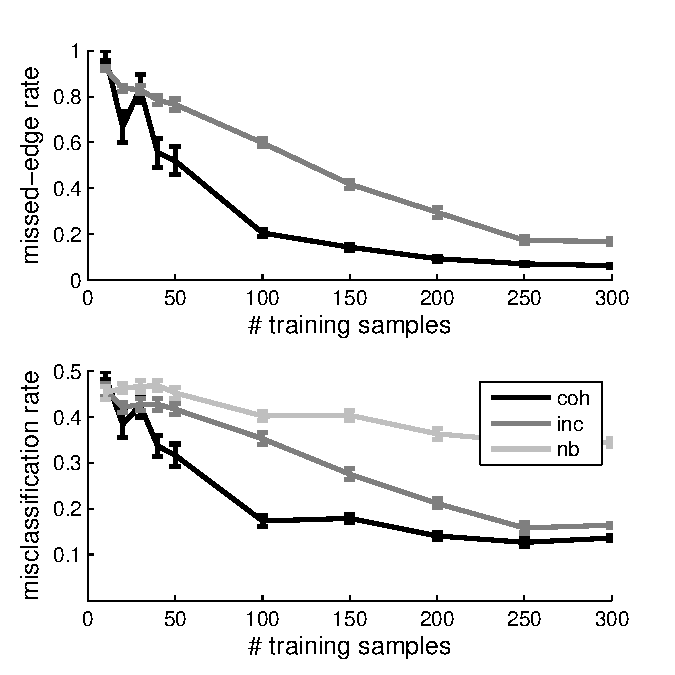
\includegraphics[width=1.0\linewidth]{../figs/homo_V70_s20_p10_q30_Lhats.pdf}
	\caption{Performance statistics as a function of sample size demonstrate that the coherent signal subgraph estimator outperforms the incoherent signal subgraph estimator, in terms of both the signal subgraph identification and classification, for nearly all $n$, using the same model as in Figure \ref{fig:4x4}.  The top panel shows the missed-edge rate for each estimator as a function of the number of training samples, $n$.  The bottom panel shows the corresponding misclassification rate for the two estimators, as well as the na\"ive Bayes plugin classifier.  Performance of all estimators improves (nearly) monotonically with $n$ for both criteria.  Error bars show standard error of the mean here and elsewhere (averaged over 20 trials; each trial used 100 samples for held-out data). Note that for most values of $n$, we have $L_{\mhb{\pi}} \geq \mh{L}_{nb} \geq \mh{L}_{inc} \geq \mh{L}_{coh} \geq L_*$. Legend: ``inc:'' incoherent; ``coh:'' coherent; ``nb:'' na\"ive Bayes.}
	\label{fig:homo}
\end{figure}


\subsection{Relative Efficiency} % (fold)
\label{sub:relative_efficiencies}

The above numerical results suggest that the coherent estimator outperforms the incoherent estimator almost always.  However, that result is a function of both the model, $\mc{M}_V$ (which includes the number of vertices), and the number of samples $n$.  %Unfortunately, analytical results computing the finite sample efficiencies of each estimator are beyond our means, as is an exhaustive treatment.  Nonetheless, 
Figure \ref{fig:RE} explicitly shows that the relative performance of an estimator for a particular model changes as a function of the number of samples.  More specifically, for small $n$, the incoherent estimator yields better performance, as indicated by the relative rate and relative efficiency being above one.  However, with more samples, when the signal subgraph is coherent, the coherent estimator will eventually outperform the incoherent one.  At infinite samples, since both estimators are consistent, they will yield identical results: the truth.  

Thus, to choose which estimator will likely achieve the best performance, knowledge of the model, $\mc{M}_V(m,s;\pi,p,q)$, is insufficient; rather, both the model and the number of samples must be known a priori.  

\begin{figure}[htbp]
	\centering
		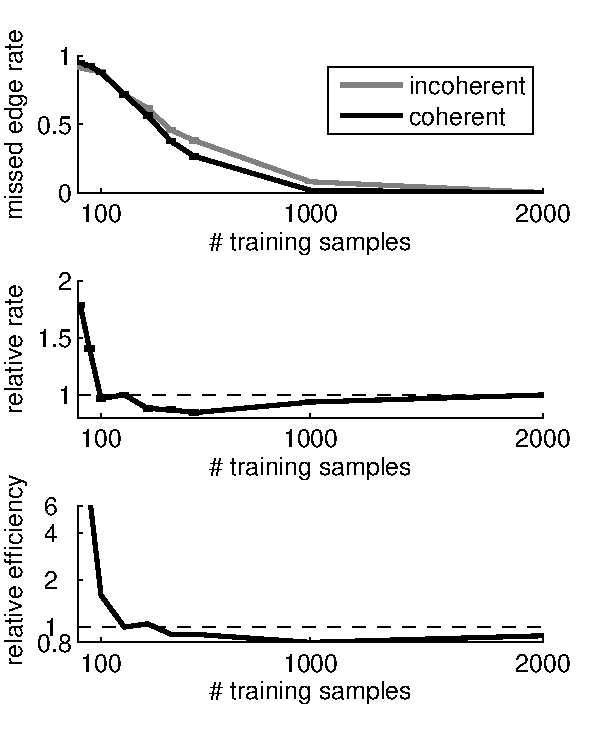
\includegraphics[width=0.8\linewidth]{../figs/RE_V30_s5_p10_q20.pdf}
	\caption{The relative performance of the coherent and incoherent estimators is a function not just of the model, but also the number of samples.  Specifically, for the model $\mc{M}_{30}(1,5;0.5,0.1,0.2)$, we compute the missed-edge rates for both the incoherent estimator (gray line) and the coherent estimator (black line).  The top panel shows that for small sample size the incoherent estimator achieves a better (lower) missed-edge rate than the coherent estimator. However, the incoherent estimator's convergence rate is slower, therefore, the coherent estimator catches up and outperforms the incoherent estimator; until both eventually converge at the truth.  The middle and bottom panels show the relative rate and efficiency curves for this model. Note that the curves dip below unity, and then converge to unity, as they must, because both estimators are consistent. }
	\label{fig:RE}
\end{figure}


\subsection{Estimating the hyper-parameters} % (fold)
\label{sub:estimating_the_hyper_parameters}

In the above analyses the hyper-parameters, both the number of signal edges $s$ and signal vertices $m$, were known.  In practice while one might have a preliminary guess of the range of these hyper-parameters, they will at times be unknown.  We can therefore use a cross-validation technique to search over the space of all reasonable combinations of $s$ and $m$, and choose the best performing combination.  Figure \ref{fig:coherent} shows one such simulation depicting several key features.  The top panel shows the misclassification rate as a function of the log of the size of the signal subgraph, $s$, for the incoherent classifier.  Although the true size is $s=20$, the best performing estimate is $\mh{s}_{inc}=23$. This is a relatively standard result in model selection: the best performer will include a few extra dimensions because adding a few uninformative features is less costly than missing a few informative features \cite{Jain2000}.  This intuition is further reified by the U-shape of the misclassification curve on a log scale: including many non-signal edges is less detrimental than excluding a few signal edges.

The bottom panel shows the performance by varying both $m$ and $s$, which has a ``banded'' like structure, indicating that the performance is relatively robust to small changes in $m$.  Moreover, the best performing pair achieved $\mh{L}_{coh}=0.13$ (which is equal to the Bayes error) with $\mh{m}_{coh}=1$ and $\mh{s}_{coh}=24$, suggesting that $n$ was sufficiently large to correctly find the true signal vertex, and further corroborating the ``better safe than sorry'' attitude to selecting the signal vertices. 

\begin{figure}[htbp]
	\centering
		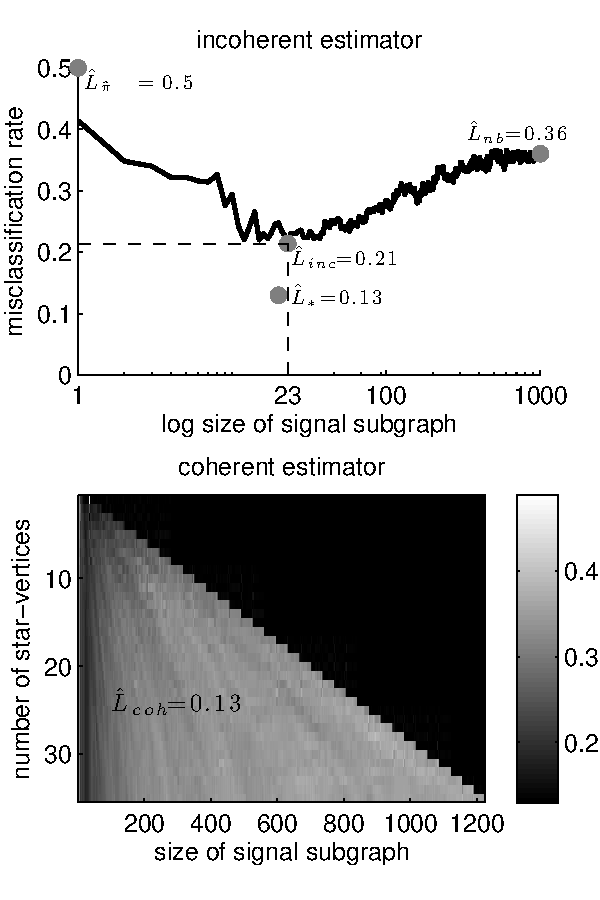
\includegraphics[width=0.8\linewidth]{../figs/coherent_image_V70_s20_p10_q30_nTr200_nTe500.pdf}
	\caption{ When constraints on the number of signal edges ($s$) or signal vertices ($m$) are unknown, a search over these hyperparameters can yield estimates $\mh{s}$ and $\mh{m}$.  Both panels depict held-out cross-validation error as a function of varying these parameters for the same model as in Figure 4, using 200 training samples and 500 test samples, with $m=1$ and $s=20$.  The top panel depicts misclassification rate of the incoherent estimator as a function of the number of edges on a log scale, with the best performing classifier achieving $\mh{L}_{inc}=0.21$. Note that in this simulation, while $s=20< \mh{s}_{inc}=23$.  This ``conservatism'' is typical and appropriate in many model selection situations.  The bottom panel shows $\mh{L}_{coh}$ as a function of both $m'$ and $s'$.  For this simulation, $\mh{m}_{coh}=1$ and $\mh{s}_{coh}=24$, further corroborating the conservative stance on model selection. Note that $L_{\mb{\pi}} \geq \mh{L}_{nb} \geq \mh{L}_{inc} \geq \mh{L}_{coh} \geq L_*$ as one would hope for this coherent simulation.  Incidentally, the coherent classifier achieved Bayes error here.}
	\label{fig:coherent}
\end{figure}


% subsection estimating_the_hyper_parameters (end)

\subsection{MR Connectome Classification} % (fold)
\label{sub:mr_connectome_classification}

A connectome may be defined as the complete set of connections of the brain \cite{Sporns2010}.  MR connectomes utilize multi-modal Magnetic Resonance (MR) imaging to determine both the vertex and edge set for each individual \cite{Hagmann2010}.  This section investigates the utility of the above described classifiers on data collected for the Baltimore Longitudinal Study of Aging, as described previously \cite{OHBM10}.  Briefly, 49 subjects (25 male, 24 female) underwent a DTI protocol; simple graphs with 70 vertices (each vertex corresponding to a neuroanatomical gyral region as defined by \cite{Desikan2006}) were estimated using the MRCAP layout \cite{BMES10}.  Lacking strong priors on either the number of signal edges or signal vertices in the signal subgraph (or even whether a signal subgraph existed), we searched over a large space of hyper-parameters using cross-validated misclassification performance as our metric of success (Figure \ref{fig:data}).  The na\"ive Bayes classifier---which assumes the signal subgraph is the whole edge set, $\mhc{S}_{nb}=\mc{E}$---performs marginally better than chance: $\mh{L}_{nb}=0.41$ (p-value $\approx 0.05$ assessed by a permutation test).  With a relatively small number of incoherent edges---$\mh{s}_{inc}=10$---the incoherent classifier (top left panel) achieves $\mh{L}_{inc}=0.27$, significantly better than chance (p-value $<0.0007$), but not significantly better than the na\"ive Bayes classifier (using McNemar's test).  The coherent classifier achieved a minimum of $\mh{L}_{coh}=0.16$ (top right and middle panels), not significantly better than the incoherent classifier, but significantly better than both chance and the na\"ive Bayes classifier (p-values $<10^{-5}$ and $<0.004$, respectively; note that no multiple hypothesis testing corrections were performed).  This improved performance upon using the coherent classifier suggests that signal subgraph is coherent. Using $\mh{m}_{coh}=12$ and $\mh{s}_{coh}=360$ from the best performing coherent classifier, we can estimate the signal subgraph (bottom right).  The coherogram suggests that indeed, the signal is somewhat, but not strikingly coherent (bottom right).

% subsection mr_connectome_classification (end)


\begin{figure}[htbp]
	\centering
		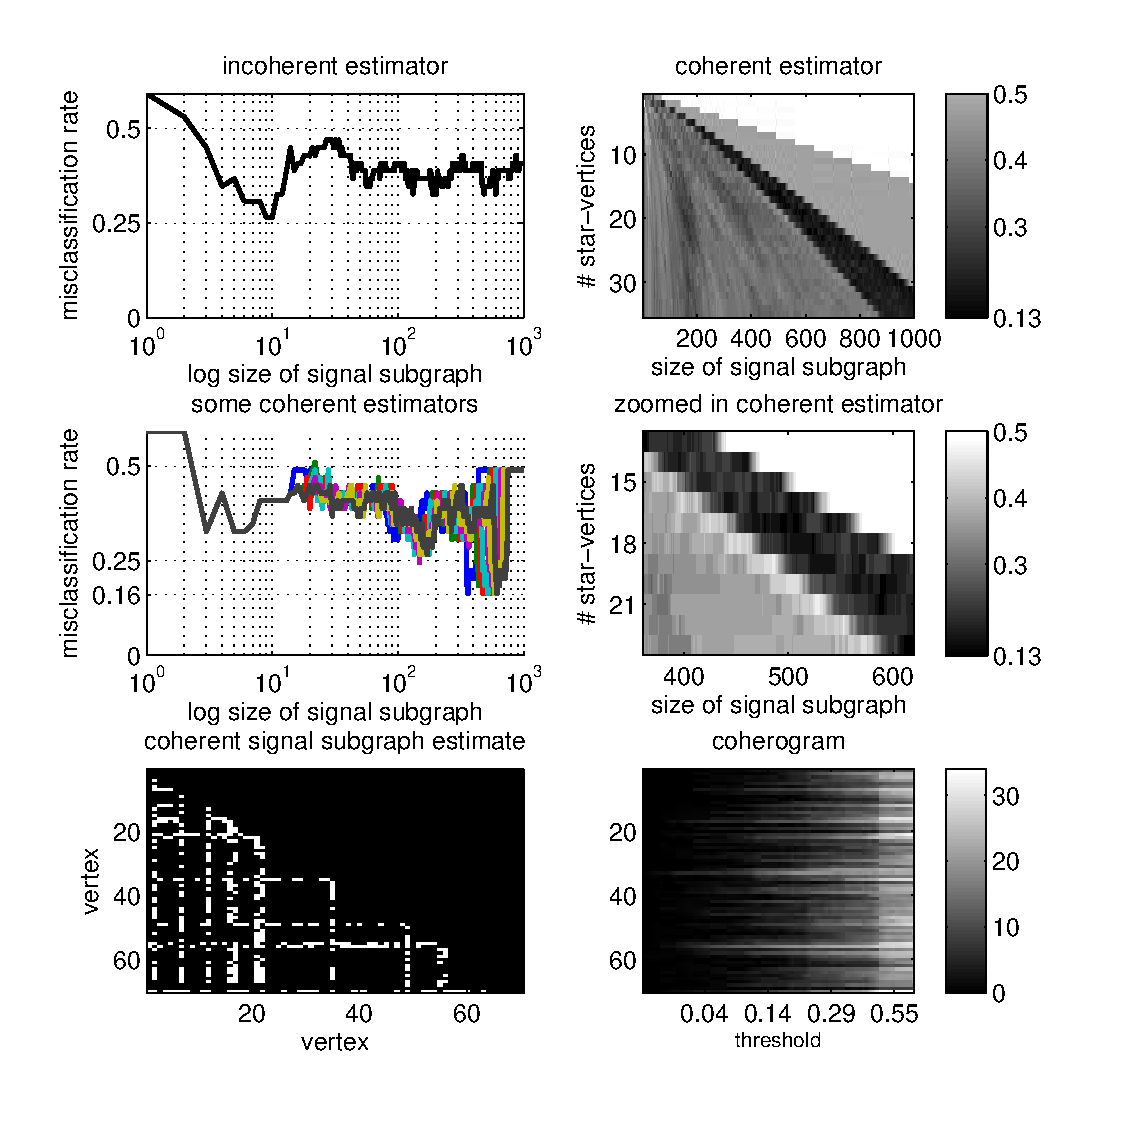
\includegraphics[width=1.0\linewidth]{../figs/BLSA0317_Count_Lhats_results.pdf}
	\caption{MR connectome sex signal subgraph estimation and analysis. By cross-validating over hyperparameters and models, we estimate that the ``best'' incoherent signal subgraph (for this inference task on these data) has $\mh{s}_{inc}=10$ and yields a misclassification rate of $\mh{L}_{inc}=0.27$, whereas the best coherent signal subgraph has $\mh{m}_{coh}=12$ and $\mh{s}_{coh}=360$, achieving $\mh{L}_{coh}=0.16$.  The top two panels depict the same information as Figure 5.  The middle two depict misclassification rate (left) for different choices of $m'$ as a function of $s'$ and (right) a zoomed in depiction of the top right panel. The bottom left panel shows the estimated signal subgraph, and the bottom right shows the coherogram.  Together, these bottom panels suggest that the signal subgraph for these data is neither particularly coherent or incoherent.}
	\label{fig:data}
\end{figure}

\subsection{Model Evaluation} % (fold)
\label{sub:model_checking}

Although the above coherent classifier estimated a signal subgraph, we wondered to what extent the estimated signal subgraph represented the true signal subgraph.  We address this question in two ways:  (i) synthetic data analysis and (ii) assumption checking.  

\subsubsection{Synthetic data analysis} % (fold)
\label{ssub:synthetic_data_analysis}

% subsubsection synthetic_data_analysis (end)
For the synthetic data analysis, we generated data as follows.  Given the above estimated signal subgraph, for every edge not in $\mhc{S}_{n}$, let $p_{uv|0}=p_{uv|1}=\mh{p}_{uv}$, where $\mh{p}_{uv}$ is the estimated edge probability averaging over all samples.  For all edges in $\mhc{S}_{n}$, let $p_{uv|y}=\mh{p}_{uv|y}$.  Set the priors according to the data as well: $\pi=\mh{\pi}$.  

\begin{figure*}[tb!]
	\centering
		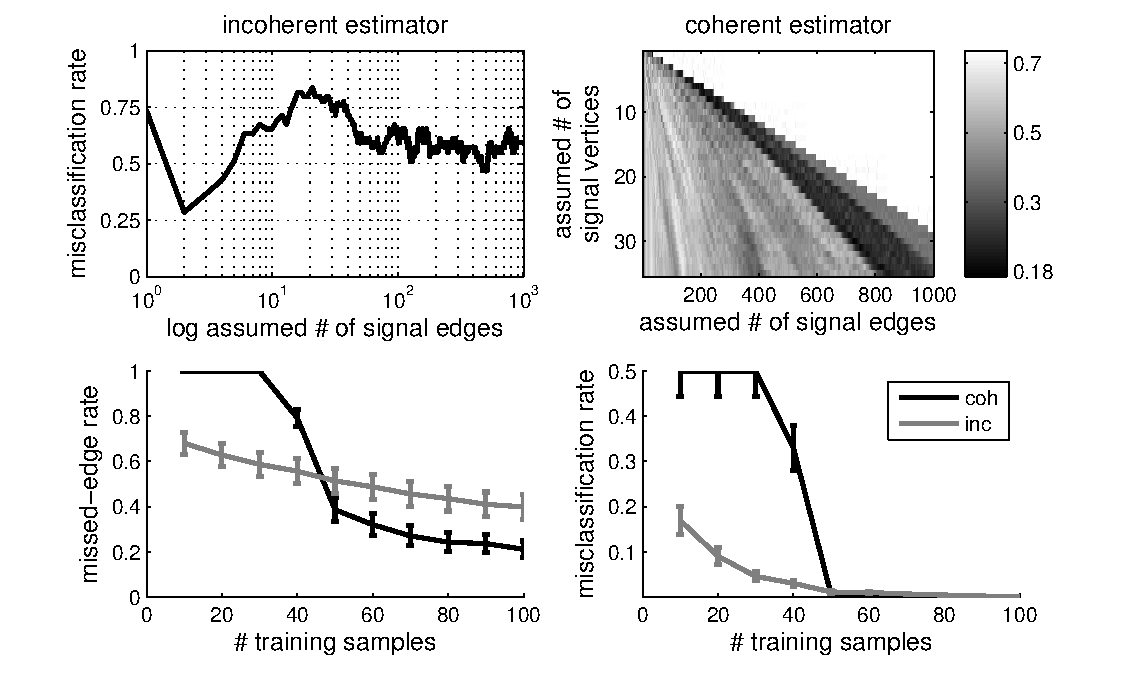
\includegraphics[width=0.7\linewidth]{../figs/BLSA0317_Count_synthetic_Lhats.pdf}
	\caption{Synthetic data analysis provides some intuition for model checking and future improvements.  The top two panels show the incoherent (left) and coherent (right) misclassification rates as a function of the hyper-parameter choices for $n=49$.  These plots look quite similar to those from Figure \ref{fig:data}, which suggests that the chosen model may be adequate.  The bottom panels show the missed-edge rate (left) and misclassification rate (right) as a function of the number of training samples.  With about 50 training samples, approximately half of the edges identified by each classifier are true edges.  Additionally, slightly more than 50 training samples seems to be sufficient for obtaining nearly perfect classification, suggesting that perhaps only a few more subjects would be sufficient to yield much greater classification performance.}
	\label{fig:synthetic}
\end{figure*}

Given this synthetic data model, we first sampled 49 data samples, 25 from class 0 and 24 from class 1, and estimated the incoherent and coherent classifier performance on a single trial (Figure \ref{fig:synthetic}, top panels).  The performance of the classifiers on the synthetic data qualitatively mirrors that of the real data, suggesting some model goodness-of-fit.  To assess what fraction of the edges in the estimated signal subgraph were reliable, even assuming a true model, we then sampled up to 100 training samples (and 100 test samples), and computed the missed-edge rate (bottom left) and misclassification rate (bottom right) as a function of the number of samples.  Given approximately 50 samples, the incoherent signal subgraph estimator correctly identifies about $40\%$ of the edges, whereas the coherent signal subgraph estimator correctly identifies about $50\%$.  This suggests that even if the model were true (which it is not) we should only believe that about half the edges in the estimated signal subgraph are in the actual signal subgraph.  Moreover, both missed-edge rate and misclassification rate exhibit a step-like function in peformance: after about 50 samples, performance dramatically improves.  This suggests that perhaps only a few more data points would be necessary to obtain greatly improved classification accuracy.  


\subsubsection{Model checking} % (fold)
\label{ssub:model_checking}

% subsubsection model_checking (end)

Checking whether edges are independent is relatively easy.  Figure \ref{fig:cov} shows the correlation coefficient between all pairs of edges in the estimated signal subgraph from the neurobiological data.  We used a spectral clustering algorithm \cite{Dhillon2001} to  more clearly highlight any significant correlations.  Several groups of edges seem to be highly  correlated.  To assess significance, we compare the distribution of correlation coefficients with the distribution of correlation coefficients obtained from the synthetic data analysis.  A two-sample Kolmogorov-Smirnov test shows that the two matrices are significantly different (p-value $\approx 0$), rejecting the null hypothesis that the edges in the real data are independent. 



\begin{figure}[htbp]
	\centering
		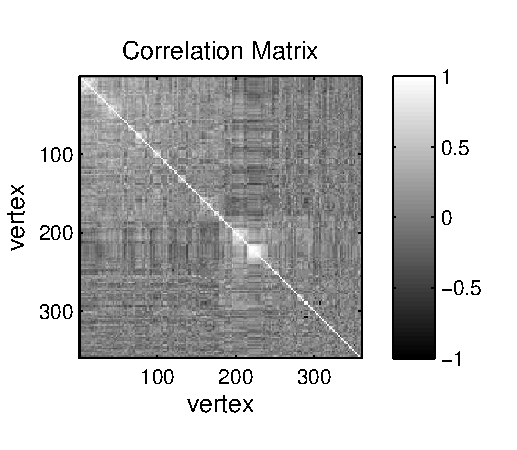
\includegraphics[width=1.0\linewidth]{../figs/BLSA0317_coclustered_corr.pdf}
	\caption{The correlation matrix between all the edges in the coherent signal subgraph estimate. Edges are organized by co-clustering to highlight any similarities.  Although most edges are uncorrelated, several groups of edges cluster, indicative of the fact that the edges are not independent (p-value of $\approx 0$ using a two-sample Kolmogorov-Smirnov test comparing the real and synthetic correlation matrices). }
	\label{fig:cov}
\end{figure}



% subsection model_checking (end)




% subsection subsection_name (end)


% subsection relative_efficiencies (end)

% section results (end)


\section{Discussion} % (fold)
\label{sec:discussion}

This work makes the following contributions. First, it introduces a novel graph/class model that admits rigorous statistical investigation.  Moreover, it presents two approaches for estimating the signal subgraph: the first using only vertex label information, the second also utilizing graph structure.  The resulting estimators have desirable asymptotic and finite sample properties, including consistency and robustness to various model misspecifications.  Third, simulated data analysis indicate that neither approach dominates the other; rather, the best approach is a function of both the model and the amount of training data. Fourth, these classifiers are applied to a connectome data set; the coherent classifier performs significantly better than both na\"ive Bayes and incoherent classifiers.  Fifth, synthetic data analysis suggests that while we can use the signal subgraph estimators to improve classification performance, we should not expect that all the edges in the estimated signal subgraph will be the true signal edges, even when the model is correct. Moreover, we might expect a drastic improvement in classification performance with only a few additional data samples.  Finally, model checking suggests that the independent edge assumption does not fit the data well.  

Collectively, the above analyses suggest a number of possible next steps.  First, collect more data.  Second, relax various assumptions, including (i) the independent edge assumption by considering conditionally independent edges \cite{Hoff02}, (ii) binary edge assumption, and (iii) labeled vertices assumption.  Third, transform a number of conjectures that have arisen due to these results into theorems.  For instance, perhaps the misclassification rate is a monotonic function of the missed-edge rate.  Fourth, (Bayesian) model-averaging to combine estimated signal subgraphs instead of picking one might improve performance (perhaps at the cost of computational resources and interpretability).  

We hope the proposed approaches will yield many applications.  To that end, all the data and code used in this work is available from the author's website, \url{jovo.me}.  

% \subsection{Related Work} % (fold)
% \label{sub:related_work}
% 
% LASSO/ENET, low-rank+sparse, other graph classification approaches (invariants, embedding, kernels) \cite{PCP10}
% 
% % subsection related_work (end)
% 
% % section discussion (end)


% \appendices
% \section{Proof of the First Zonklar Equation}
% Appendix one text goes here.
% 
% % you can choose not to have a title for an appendix
% % if you want by leaving the argument blank
% \section{}
% Appendix two text goes here.

% use section* for acknowledgement
\ifCLASSOPTIONcompsoc
  % The Computer Society usually uses the plural form
  \section*{Acknowledgments}
\else
  % regular IEEE prefers the singular form
  \section*{Acknowledgment}
\fi


% Can use something like this to put references on a page
% by themselves when using endfloat and the captionsoff option.
\ifCLASSOPTIONcaptionsoff
  \newpage
\fi


\bibliography{/Users/jovo/Research/latex/library}
\bibliographystyle{IEEEtran}

\begin{IEEEbiography}{Joshua T. Vogelstein}
Joshua T. Vogelstein received the B.S degree in biomedical engineering from Washington University in St. Louis, MO in 2002, the M.S. degree in applied mathematics and statistics from Johns Hopkins University (JHU) in Baltimore, MD in 2009, and the Ph.D. degree in neuroscience from Johns Hopkins School of Medicine in Baltimore, MD in 2009.  He is currently a postdoctoral fellow in the Department of Applied Mathematics and Statistics at JHU, with a joint appointment in the Human Language Technology Center of Excellence.  His research interests primarily include statistical connectomics, including theory and applications for high-dimensional graph-valued data. His research has been featured in a number of prominent scientific and engineering journals including Annals of Applied Statistics, IEEE Transactions on Neural Systems and Rehabilitation Engineering, and Nature Neuroscience.

\end{IEEEbiography}

% if you will not have a photo at all:
\begin{IEEEbiographynophoto}{William R. Gray}
William R. Gray graduated from Vanderbilt University in 2003 with a Bachelor’s degree in electrical engineering, and received his MS in electrical engineering in 2005 from the University of Southern California.  Currently, Will is a PhD student in electrical engineering at Johns Hopkins University, where he is conducting research in the areas of connectivity, signal and image processing, and machine learning.  He is also a member of the technical staff at the Johns Hopkins University Applied Physics Laboratory, where he manages projects in the Biomedicine and Undersea Warfare business areas.  Will is a member of IEEE, Eta Kappa Nu, and Tau Beta Pi
\end{IEEEbiographynophoto}

% insert where needed to balance the two columns on the last page with
% biographies
%\newpage

\begin{IEEEbiographynophoto}{R. Jacob Vogelstein}
R. Jacob Vogelstein received the Sc.B. degree in neuroengineering from Brown University, Providence, RI, and the Ph.D. degree in biomedical engineering from the Johns Hopkins University School of Medicine, Baltimore, MD.  He currently oversees the Applied Neuroscience programs at the Johns Hopkins University (JHU) Applied Physics Laboratory as an Assistant Program Manager, and has an appointment as an Assistant Research Professor at the JHU Whiting School of Engineering’s Department of Electrical and Computer Engineering. He has worked on neuroscience technology for over a decade, focusing primarily on neuromorphic systems and closed-loop brain–machine interfaces. His research has been featured in a number of prominent scientific and engineering journals including the IEEE Transactions on Neural Systems and Rehabilitation Engineering, the IEEE Transactions on Biomedical Circuits and Systems, and the IEEE Transactions on Neural Networks.  
\end{IEEEbiographynophoto}

\begin{IEEEbiography}{Carey E. Priebe}
Carey E. Priebe received the B.S. degree in mathematics from Purdue University in 1984, the M.S. degree in computer science from San Diego State University in 1988, and the Ph.D. degree in information technology (computational statistics) from George Mason University in 1993. From 1985 to 1994 he worked as a mathematician and scientist in the US Navy research and development laboratory system. Since 1994 he has been a professor in the Department of Applied Mathematics and Statistics, Whiting School of Engineering, Johns Hopkins University, Baltimore, Maryland. At Johns Hopkins, he holds joint appointments in the Department of Computer Science, the Department of Electrical and Computer Engineering, the Center for Imaging Science, the Human Language Technology Center of Excellence, and the Whitaker Biomedical Engineering Institute. He is a past President of the Interface Foundation of North America - Computing Science \& Statistics, a past Chair of the American Statistical Association Section on Statistical Computing, a past Vice President of the International Association for Statistical Computing, and on the editorial boards of Journal of Computational and Graphical Statistics, Computational Statistics and Data Analysis, and Computational Statistics. His research interests include computational statistics, kernel and mixture estimates, statistical pattern recognition, statistical image analysis, dimensionality reduction, model selection, and statistical inference for high-dimensional and graph data. He is a Senior Member of the IEEE, a Lifetime Member of the Institute of Mathematical Statistics, an Elected Member of the International Statistical Institute, and a Fellow of the American Statistical Association.
\end{IEEEbiography}

% Can be used to pull up biographies so that the bottom of the last one
% is flush with the other column.
% \enlargethispage{-5in}

\end{document}
